El segundo nodo se encargará directamente de notificar al conductor cuando algún
comportamiento es errático o peligroso. Entre otras tareas, este nodo se encarga
de monitorizar el estado del conductor (y detectar posibles signos de somnolencia)
y emitir avisos luminosos y sonoros cuando se produzcan situaciones de riesgo.

Este sistema cuenta con cinco tareas en tiempo real y tres objetos protegidos: el
primero recoge datos sobre síntomas como son la inclinación de la cabeza o el
giro del volante; el segundo, recoge información sobre si el conductor está
sujetando o no el volante; y el tercero establecerá el modo de funcionamiento de
los avisos del sistema. Con respecto a las tareas, se tiene:

\begin{enumerate}
  \item \texttt{Inclinación cabeza} -- cada $\numprint[ms]{600}$, leerá el valor del
        giroscopio integrado para actualizar los datos de las posiciones $X$ e $Y$,
        en el objeto protegido \texttt{Síntomas 1}.
  \item \texttt{Detección volantazos} -- cada $\numprint[ms]{400}$ el sistema leerá
        el valor de la posición del volante y actualizará el dato recogido en
        \texttt{Síntomas 1}. Si durante dos lecturas consecutivas la diferencia
        entre las posiciones del volante es de más de $150$ y la velocidad es mayor
        a $70\nicefrac{km}{h}$ entonces se considera que el conductor está dando
        volantazos. Si pasan más de 5 segundos sin que se repita esa situación,
        el conductor estará conduciendo normalmente.
  \item \texttt{Relax al volante} -- cada $\numprint[ms]{500}$, el sistema actualizará
        en \texttt{Síntomas 2} si el conductor está sujetando o no el volante.
  \item \texttt{Detección pulsador} -- tarea esporádica que será activada desde la rutina
        de tratamiento de interrupciones \textit{hardware} que establecerá cíclicamente
        el modo de funcionamiento del sistema en el objeto protegido \texttt{Modo}.
  \item \texttt{Riesgos} -- cada $\numprint[ms]{300}$, el sistema evaluará los datos
        recogidos en los objetos protegidos \texttt{Síntomas 1}, \texttt{Síntomas 2} y \texttt{Modo} y
        establecerá el nivel de alarma para con el conductor. Dicha detección de riesgos
        viene definida por la siguiente secuencia:
        \begin{itemize}
          \item $S_1$ -- si el conductor presenta una inclinación de la cabeza en los ejes $X, Y$
                de más de $20\degree$ y no tiene sujeto el volante se considera que está
                manipulando el móvil u otro aparato. Se activa la luz amarilla y se
                emite un pitido nivel 1.
          \item $S_2$ -- si la inclinación de la cabeza es $X > 20\degree | Y > 20\degree$, el volante
                está agarrado y la velocidad es mayor de $70\nicefrac{km}{h}$ se interpreta
                que el conductor no está prestando atención a la carretera y se encenderá la
                luz amarilla.
          \item $S_3$ -- si se detecta una inclinación en el eje $X$ de más de $30\degree$ y el
                conductor está dando volantazos se interpreta como síntoma de somnolencia.
                Se encenderá la luz amarilla y se emitirá un pitido nivel 2.
          \item $S_4$ -- si se dan simultáneamente dos de los riegos anteriores se pasa a estar en
                \textbf{NIVEL 2} de alerta y se encenderá la luz roja y emitirá un pitido
                nivel 2.
          \item $S_5$ -- si se produce un riesgo \textbf{NIVEL 2} y la distancia con el vehículo
                precedente es menor al 50\% de la distancia de seguridad recomendada, se
                estará ante una situación de \textbf{EMERGENCIA} y se activará el freno,
                junto con todo lo anterior.
        \end{itemize}
\end{enumerate}

La evaluación de riesgos se puede modelar mediante el diagrama \ref{fig:risks-diagram}:

\begin{figure}[H]
  \begin{tikzpicture}[->,>=stealth',shorten >=1pt,auto,node distance=3cm,
      scale = 1,transform shape]

    \node[state] (Riesgos) {Riesgos};
    \node[state] (Luz amarilla) [below right =of Riesgos] {Luz amarilla};
    \node[state] (Pitido) [right =of Luz amarilla] {Pitido};
    \node[state] (Luz roja) [right =of Pitido] {Luz roja};
    \node[state] (RL2) [below right =of Luz amarilla] {Riesgo lvl. 2};
    \node[state] (Emergencia) [right =of RL2] {Emergencia};

    \path (Riesgos) edge[bend right] node {$S_1, S_2, S_3$} (Luz amarilla);
    \path (Luz amarilla) edge node {$S_1\left(1\right), S_3\left(2\right)$} (Pitido);
    \path (Luz amarilla) edge[bend right] node {$S_4 = \sum_i S_i \geq 2$} (RL2);
    \path (RL2) edge node {} (Luz roja);
    \path (Luz roja) edge node {$\left(2\right)$} (Pitido);
    \path (RL2) edge node {$d \leq 50\% \cdot d_{\min}$} (Emergencia);

  \end{tikzpicture}
  \caption{Diagrama que modela la interpretación de los riesgos, descritos en la enumeración
    anterior ($S_i$). La intensidad del pitido va acompañada entre paréntesis del síntoma
    que lo activa (por ejemplo, $S_1\left(1\right)$ indica una intensidad de pitido nivel 1)
    o en solitario, si es consecuencia de acciones en cadena.}
  \label{fig:risks-diagram}
\end{figure}

Y, en general, el nodo 2 se puede representar mediante la figura \ref{fig:node2}:

\begin{figure}[H]
  \centering
  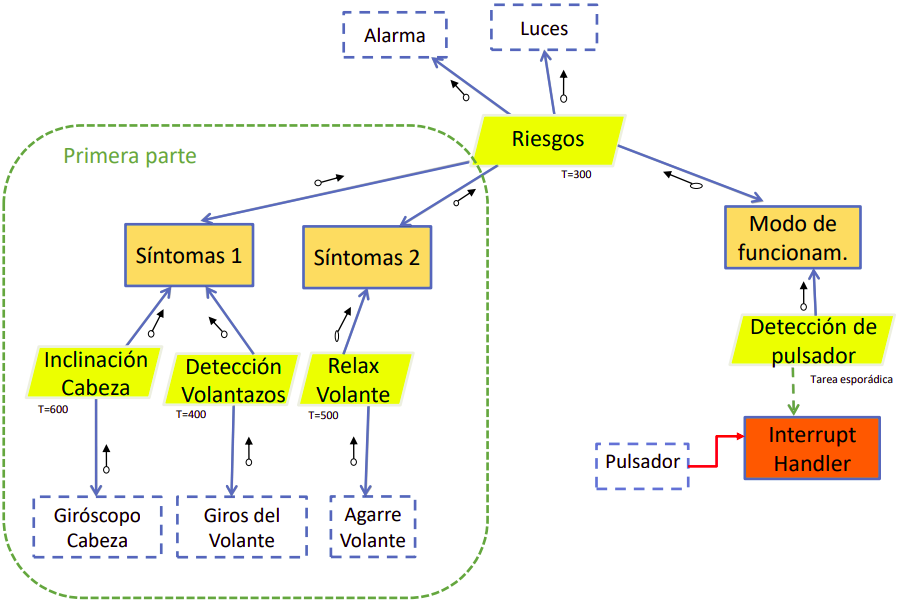
\includegraphics[width=.8\linewidth]{pictures/node2.png}
  \caption{Modelado del nodo 2 junto con sus tareas, objetos protegidos, sensores y actuadores.}
  \label{fig:node2}
\end{figure}
